\begin{minipage}[b]{0.15\linewidth}
\begin{figure}[H]                                                          
  \centering                                                             
  \begin{adjustbox}{width=1.5cm,center}                                   
  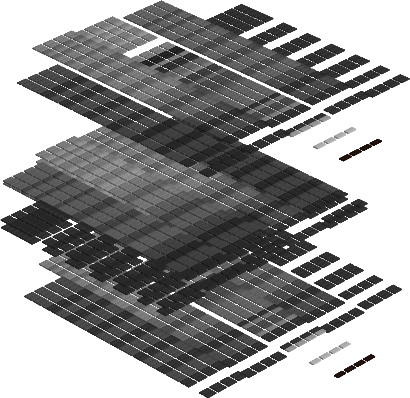
\includegraphics[width=1.5cm]{src/colorspace_colourflow/flows/colourflow_0-45.png}%           
  \end{adjustbox}                                                        
\caption*{

\begin{tikzpicture}                             
\definecolor{tempcolor}{HTML}{000000}           
\fill[tempcolor] (1 mm,0) rectangle ++(1mm,1mm);
\definecolor{tempcolor}{HTML}{000000}           
\fill[tempcolor] (2 mm,0) rectangle ++(1mm,1mm);
\definecolor{tempcolor}{HTML}{111111}           
\fill[tempcolor] (3 mm,0) rectangle ++(1mm,1mm);
\definecolor{tempcolor}{HTML}{333333}           
\fill[tempcolor] (4 mm,0) rectangle ++(1mm,1mm);
\definecolor{tempcolor}{HTML}{555555}           
\fill[tempcolor] (5 mm,0) rectangle ++(1mm,1mm);
\definecolor{tempcolor}{HTML}{777777}           
\fill[tempcolor] (6 mm,0) rectangle ++(1mm,1mm);
\definecolor{tempcolor}{HTML}{999999}           
\fill[tempcolor] (7 mm,0) rectangle ++(1mm,1mm);
\definecolor{tempcolor}{HTML}{bbbbbb}           
\fill[tempcolor] (8 mm,0) rectangle ++(1mm,1mm);
\end{tikzpicture}                               
}
\end{figure}                                                               
\end{minipage}
\hspace{0.1cm}
\begin{minipage}[b]{0.15\linewidth}
\begin{figure}[H]                                                          
  \centering                                                             
  \begin{adjustbox}{width=1.5cm,center}                                   
  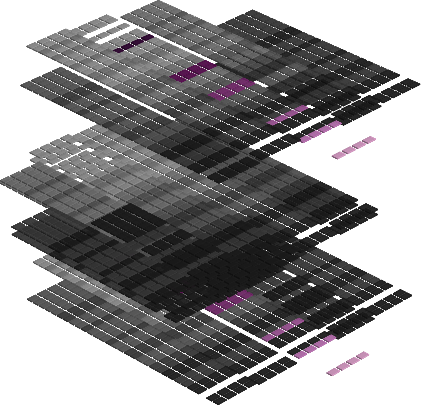
\includegraphics[width=1.5cm]{src/colorspace_colourflow/flows/colourflow_1-45.png}%           
  \end{adjustbox}                                                        
\caption*{

\begin{tikzpicture}                             
\definecolor{tempcolor}{HTML}{000000}           
\fill[tempcolor] (1 mm,0) rectangle ++(1mm,1mm);
\definecolor{tempcolor}{HTML}{111111}           
\fill[tempcolor] (2 mm,0) rectangle ++(1mm,1mm);
\definecolor{tempcolor}{HTML}{222222}           
\fill[tempcolor] (3 mm,0) rectangle ++(1mm,1mm);
\definecolor{tempcolor}{HTML}{444444}           
\fill[tempcolor] (4 mm,0) rectangle ++(1mm,1mm);
\definecolor{tempcolor}{HTML}{666666}           
\fill[tempcolor] (5 mm,0) rectangle ++(1mm,1mm);
\definecolor{tempcolor}{HTML}{888888}           
\fill[tempcolor] (6 mm,0) rectangle ++(1mm,1mm);
\definecolor{tempcolor}{HTML}{aaaaaa}           
\fill[tempcolor] (7 mm,0) rectangle ++(1mm,1mm);
\definecolor{tempcolor}{HTML}{cccccc}           
\fill[tempcolor] (8 mm,0) rectangle ++(1mm,1mm);
\end{tikzpicture}                               
}
\end{figure}                                                               
\end{minipage}
\hspace{0.1cm}
\begin{minipage}[b]{0.15\linewidth}
\begin{figure}[H]                                                          
  \centering                                                             
  \begin{adjustbox}{width=1.5cm,center}                                   
  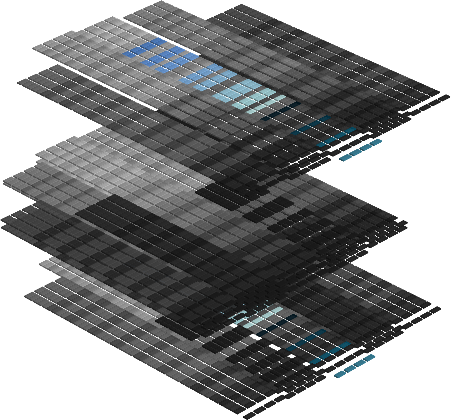
\includegraphics[width=1.5cm]{src/colorspace_colourflow/flows/colourflow_2-45.png}%           
  \end{adjustbox}                                                        
\caption*{

\begin{tikzpicture}                             
\definecolor{tempcolor}{HTML}{000000}           
\fill[tempcolor] (1 mm,0) rectangle ++(1mm,1mm);
\definecolor{tempcolor}{HTML}{222222}           
\fill[tempcolor] (2 mm,0) rectangle ++(1mm,1mm);
\definecolor{tempcolor}{HTML}{333333}           
\fill[tempcolor] (3 mm,0) rectangle ++(1mm,1mm);
\definecolor{tempcolor}{HTML}{555555}           
\fill[tempcolor] (4 mm,0) rectangle ++(1mm,1mm);
\definecolor{tempcolor}{HTML}{777777}           
\fill[tempcolor] (5 mm,0) rectangle ++(1mm,1mm);
\definecolor{tempcolor}{HTML}{999999}           
\fill[tempcolor] (6 mm,0) rectangle ++(1mm,1mm);
\definecolor{tempcolor}{HTML}{bbbbbb}           
\fill[tempcolor] (7 mm,0) rectangle ++(1mm,1mm);
\definecolor{tempcolor}{HTML}{dddddd}           
\fill[tempcolor] (8 mm,0) rectangle ++(1mm,1mm);
\end{tikzpicture}                               
}
\end{figure}                                                               
\end{minipage}
\hspace{0.1cm}
\begin{minipage}[b]{0.15\linewidth}
\begin{figure}[H]                                                          
  \centering                                                             
  \begin{adjustbox}{width=1.5cm,center}                                   
  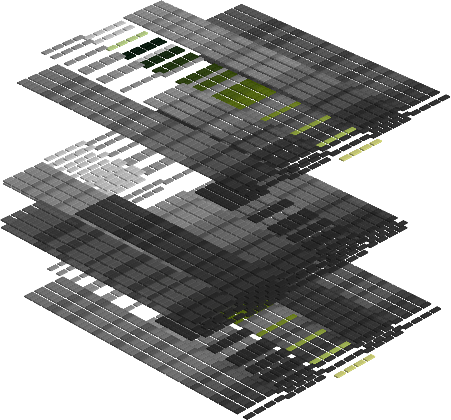
\includegraphics[width=1.5cm]{src/colorspace_colourflow/flows/colourflow_3-45.png}%           
  \end{adjustbox}                                                        
\caption*{

\begin{tikzpicture}                             
\definecolor{tempcolor}{HTML}{000000}           
\fill[tempcolor] (1 mm,0) rectangle ++(1mm,1mm);
\definecolor{tempcolor}{HTML}{333333}           
\fill[tempcolor] (2 mm,0) rectangle ++(1mm,1mm);
\definecolor{tempcolor}{HTML}{444444}           
\fill[tempcolor] (3 mm,0) rectangle ++(1mm,1mm);
\definecolor{tempcolor}{HTML}{666666}           
\fill[tempcolor] (4 mm,0) rectangle ++(1mm,1mm);
\definecolor{tempcolor}{HTML}{888888}           
\fill[tempcolor] (5 mm,0) rectangle ++(1mm,1mm);
\definecolor{tempcolor}{HTML}{aaaaaa}           
\fill[tempcolor] (6 mm,0) rectangle ++(1mm,1mm);
\definecolor{tempcolor}{HTML}{cccccc}           
\fill[tempcolor] (7 mm,0) rectangle ++(1mm,1mm);
\definecolor{tempcolor}{HTML}{eeeeee}           
\fill[tempcolor] (8 mm,0) rectangle ++(1mm,1mm);
\end{tikzpicture}                               
}
\end{figure}                                                               
\end{minipage}
\hspace{0.1cm}
\begin{minipage}[b]{0.15\linewidth}
\begin{figure}[H]                                                          
  \centering                                                             
  \begin{adjustbox}{width=1.5cm,center}                                   
  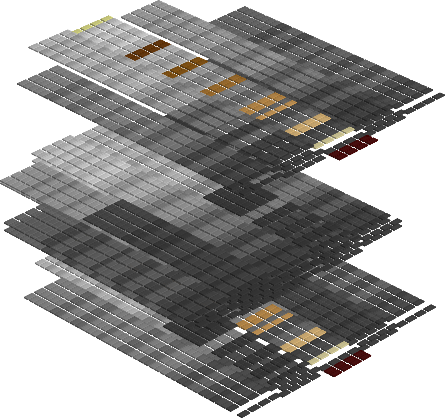
\includegraphics[width=1.5cm]{src/colorspace_colourflow/flows/colourflow_4-45.png}%           
  \end{adjustbox}                                                        
\caption*{

\begin{tikzpicture}                             
\definecolor{tempcolor}{HTML}{000000}           
\fill[tempcolor] (1 mm,0) rectangle ++(1mm,1mm);
\definecolor{tempcolor}{HTML}{444444}           
\fill[tempcolor] (2 mm,0) rectangle ++(1mm,1mm);
\definecolor{tempcolor}{HTML}{555555}           
\fill[tempcolor] (3 mm,0) rectangle ++(1mm,1mm);
\definecolor{tempcolor}{HTML}{777777}           
\fill[tempcolor] (4 mm,0) rectangle ++(1mm,1mm);
\definecolor{tempcolor}{HTML}{999999}           
\fill[tempcolor] (5 mm,0) rectangle ++(1mm,1mm);
\definecolor{tempcolor}{HTML}{bbbbbb}           
\fill[tempcolor] (6 mm,0) rectangle ++(1mm,1mm);
\definecolor{tempcolor}{HTML}{dddddd}           
\fill[tempcolor] (7 mm,0) rectangle ++(1mm,1mm);
\definecolor{tempcolor}{HTML}{ffffff}           
\fill[tempcolor] (8 mm,0) rectangle ++(1mm,1mm);
\end{tikzpicture}                               
}
\end{figure}                                                               
\end{minipage}
\hspace{0.1cm}
\begin{minipage}[b]{0.15\linewidth}
\begin{figure}[H]                                                          
  \centering                                                             
  \begin{adjustbox}{width=1.5cm,center}                                   
  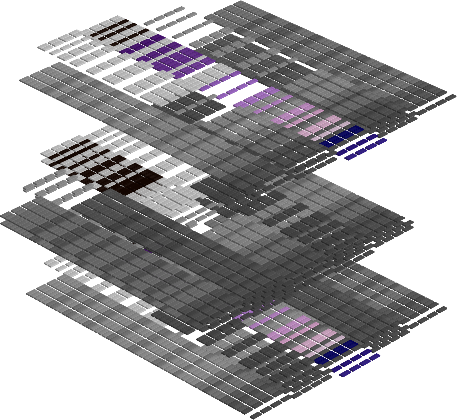
\includegraphics[width=1.5cm]{src/colorspace_colourflow/flows/colourflow_5-45.png}%           
  \end{adjustbox}                                                        
\caption*{

\begin{tikzpicture}                             
\definecolor{tempcolor}{HTML}{000000}           
\fill[tempcolor] (1 mm,0) rectangle ++(1mm,1mm);
\definecolor{tempcolor}{HTML}{555555}           
\fill[tempcolor] (2 mm,0) rectangle ++(1mm,1mm);
\definecolor{tempcolor}{HTML}{666666}           
\fill[tempcolor] (3 mm,0) rectangle ++(1mm,1mm);
\definecolor{tempcolor}{HTML}{888888}           
\fill[tempcolor] (4 mm,0) rectangle ++(1mm,1mm);
\definecolor{tempcolor}{HTML}{aaaaaa}           
\fill[tempcolor] (5 mm,0) rectangle ++(1mm,1mm);
\definecolor{tempcolor}{HTML}{cccccc}           
\fill[tempcolor] (6 mm,0) rectangle ++(1mm,1mm);
\definecolor{tempcolor}{HTML}{eeeeee}           
\fill[tempcolor] (7 mm,0) rectangle ++(1mm,1mm);
\definecolor{tempcolor}{HTML}{190700}           
\fill[tempcolor] (8 mm,0) rectangle ++(1mm,1mm);
\end{tikzpicture}                               
}
\end{figure}                                                               
\end{minipage}
\hspace{0.1cm}
\begin{minipage}[b]{0.15\linewidth}
\begin{figure}[H]                                                          
  \centering                                                             
  \begin{adjustbox}{width=1.5cm,center}                                   
  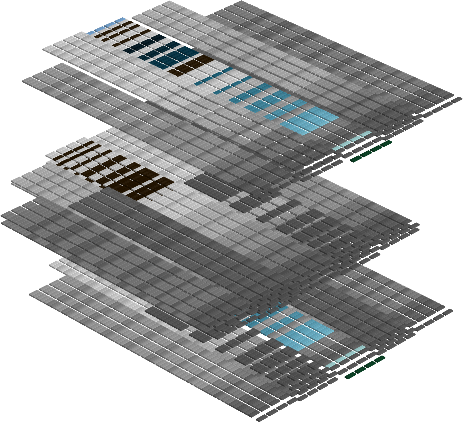
\includegraphics[width=1.5cm]{src/colorspace_colourflow/flows/colourflow_6-45.png}%           
  \end{adjustbox}                                                        
\caption*{

\begin{tikzpicture}                             
\definecolor{tempcolor}{HTML}{000000}           
\fill[tempcolor] (1 mm,0) rectangle ++(1mm,1mm);
\definecolor{tempcolor}{HTML}{666666}           
\fill[tempcolor] (2 mm,0) rectangle ++(1mm,1mm);
\definecolor{tempcolor}{HTML}{777777}           
\fill[tempcolor] (3 mm,0) rectangle ++(1mm,1mm);
\definecolor{tempcolor}{HTML}{999999}           
\fill[tempcolor] (4 mm,0) rectangle ++(1mm,1mm);
\definecolor{tempcolor}{HTML}{bbbbbb}           
\fill[tempcolor] (5 mm,0) rectangle ++(1mm,1mm);
\definecolor{tempcolor}{HTML}{dddddd}           
\fill[tempcolor] (6 mm,0) rectangle ++(1mm,1mm);
\definecolor{tempcolor}{HTML}{ffffff}           
\fill[tempcolor] (7 mm,0) rectangle ++(1mm,1mm);
\definecolor{tempcolor}{HTML}{2a1800}           
\fill[tempcolor] (8 mm,0) rectangle ++(1mm,1mm);
\end{tikzpicture}                               
}
\end{figure}                                                               
\end{minipage}
\hspace{0.1cm}
\begin{minipage}[b]{0.15\linewidth}
\begin{figure}[H]                                                          
  \centering                                                             
  \begin{adjustbox}{width=1.5cm,center}                                   
  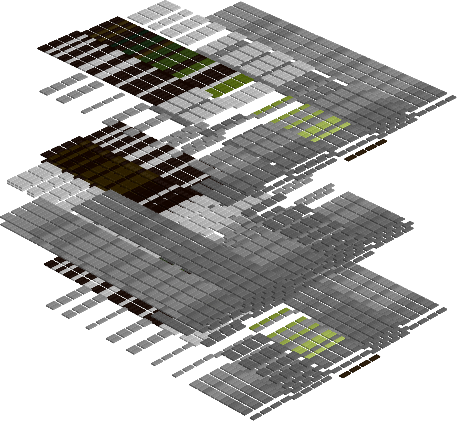
\includegraphics[width=1.5cm]{src/colorspace_colourflow/flows/colourflow_7-45.png}%           
  \end{adjustbox}                                                        
\caption*{

\begin{tikzpicture}                             
\definecolor{tempcolor}{HTML}{000000}           
\fill[tempcolor] (1 mm,0) rectangle ++(1mm,1mm);
\definecolor{tempcolor}{HTML}{777777}           
\fill[tempcolor] (2 mm,0) rectangle ++(1mm,1mm);
\definecolor{tempcolor}{HTML}{888888}           
\fill[tempcolor] (3 mm,0) rectangle ++(1mm,1mm);
\definecolor{tempcolor}{HTML}{aaaaaa}           
\fill[tempcolor] (4 mm,0) rectangle ++(1mm,1mm);
\definecolor{tempcolor}{HTML}{cccccc}           
\fill[tempcolor] (5 mm,0) rectangle ++(1mm,1mm);
\definecolor{tempcolor}{HTML}{eeeeee}           
\fill[tempcolor] (6 mm,0) rectangle ++(1mm,1mm);
\definecolor{tempcolor}{HTML}{190700}           
\fill[tempcolor] (7 mm,0) rectangle ++(1mm,1mm);
\definecolor{tempcolor}{HTML}{3b2900}           
\fill[tempcolor] (8 mm,0) rectangle ++(1mm,1mm);
\end{tikzpicture}                               
}
\end{figure}                                                               
\end{minipage}
\hspace{0.1cm}
\begin{minipage}[b]{0.15\linewidth}
\begin{figure}[H]                                                          
  \centering                                                             
  \begin{adjustbox}{width=1.5cm,center}                                   
  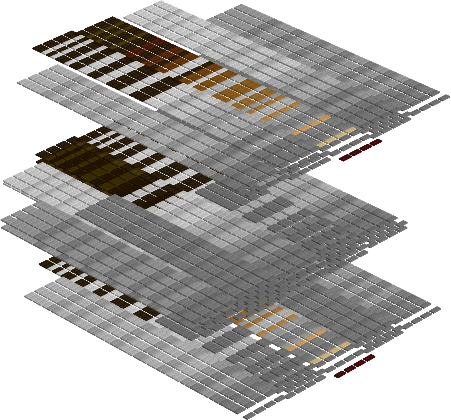
\includegraphics[width=1.5cm]{src/colorspace_colourflow/flows/colourflow_8-45.png}%           
  \end{adjustbox}                                                        
\caption*{

\begin{tikzpicture}                             
\definecolor{tempcolor}{HTML}{000000}           
\fill[tempcolor] (1 mm,0) rectangle ++(1mm,1mm);
\definecolor{tempcolor}{HTML}{888888}           
\fill[tempcolor] (2 mm,0) rectangle ++(1mm,1mm);
\definecolor{tempcolor}{HTML}{999999}           
\fill[tempcolor] (3 mm,0) rectangle ++(1mm,1mm);
\definecolor{tempcolor}{HTML}{bbbbbb}           
\fill[tempcolor] (4 mm,0) rectangle ++(1mm,1mm);
\definecolor{tempcolor}{HTML}{dddddd}           
\fill[tempcolor] (5 mm,0) rectangle ++(1mm,1mm);
\definecolor{tempcolor}{HTML}{ffffff}           
\fill[tempcolor] (6 mm,0) rectangle ++(1mm,1mm);
\definecolor{tempcolor}{HTML}{2a1800}           
\fill[tempcolor] (7 mm,0) rectangle ++(1mm,1mm);
\definecolor{tempcolor}{HTML}{4c3a00}           
\fill[tempcolor] (8 mm,0) rectangle ++(1mm,1mm);
\end{tikzpicture}                               
}
\end{figure}                                                               
\end{minipage}
\hspace{0.1cm}
\begin{minipage}[b]{0.15\linewidth}
\begin{figure}[H]                                                          
  \centering                                                             
  \begin{adjustbox}{width=1.5cm,center}                                   
  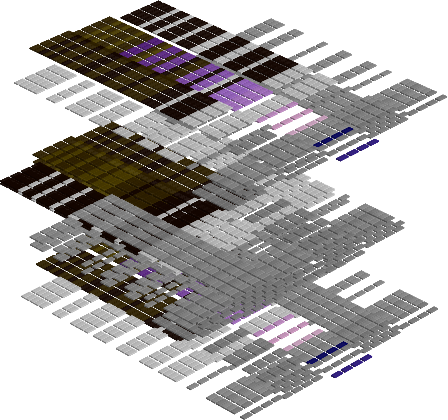
\includegraphics[width=1.5cm]{src/colorspace_colourflow/flows/colourflow_9-45.png}%           
  \end{adjustbox}                                                        
\caption*{

\begin{tikzpicture}                             
\definecolor{tempcolor}{HTML}{000000}           
\fill[tempcolor] (1 mm,0) rectangle ++(1mm,1mm);
\definecolor{tempcolor}{HTML}{999999}           
\fill[tempcolor] (2 mm,0) rectangle ++(1mm,1mm);
\definecolor{tempcolor}{HTML}{aaaaaa}           
\fill[tempcolor] (3 mm,0) rectangle ++(1mm,1mm);
\definecolor{tempcolor}{HTML}{cccccc}           
\fill[tempcolor] (4 mm,0) rectangle ++(1mm,1mm);
\definecolor{tempcolor}{HTML}{eeeeee}           
\fill[tempcolor] (5 mm,0) rectangle ++(1mm,1mm);
\definecolor{tempcolor}{HTML}{190700}           
\fill[tempcolor] (6 mm,0) rectangle ++(1mm,1mm);
\definecolor{tempcolor}{HTML}{3b2900}           
\fill[tempcolor] (7 mm,0) rectangle ++(1mm,1mm);
\definecolor{tempcolor}{HTML}{5d4b00}           
\fill[tempcolor] (8 mm,0) rectangle ++(1mm,1mm);
\end{tikzpicture}                               
}
\end{figure}                                                               
\end{minipage}
\hspace{0.1cm}
\begin{minipage}[b]{0.15\linewidth}
\begin{figure}[H]                                                          
  \centering                                                             
  \begin{adjustbox}{width=1.5cm,center}                                   
  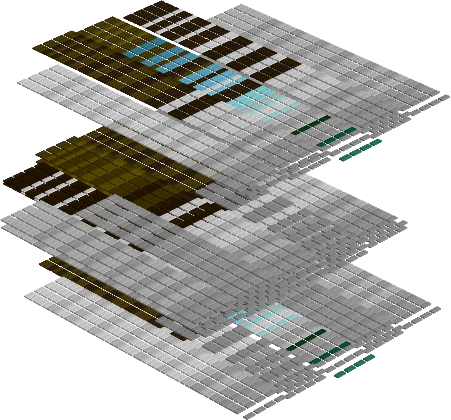
\includegraphics[width=1.5cm]{src/colorspace_colourflow/flows/colourflow_10-45.png}%           
  \end{adjustbox}                                                        
\caption*{

\begin{tikzpicture}                             
\definecolor{tempcolor}{HTML}{000000}           
\fill[tempcolor] (1 mm,0) rectangle ++(1mm,1mm);
\definecolor{tempcolor}{HTML}{aaaaaa}           
\fill[tempcolor] (2 mm,0) rectangle ++(1mm,1mm);
\definecolor{tempcolor}{HTML}{bbbbbb}           
\fill[tempcolor] (3 mm,0) rectangle ++(1mm,1mm);
\definecolor{tempcolor}{HTML}{dddddd}           
\fill[tempcolor] (4 mm,0) rectangle ++(1mm,1mm);
\definecolor{tempcolor}{HTML}{ffffff}           
\fill[tempcolor] (5 mm,0) rectangle ++(1mm,1mm);
\definecolor{tempcolor}{HTML}{2a1800}           
\fill[tempcolor] (6 mm,0) rectangle ++(1mm,1mm);
\definecolor{tempcolor}{HTML}{4c3a00}           
\fill[tempcolor] (7 mm,0) rectangle ++(1mm,1mm);
\definecolor{tempcolor}{HTML}{6e5c00}           
\fill[tempcolor] (8 mm,0) rectangle ++(1mm,1mm);
\end{tikzpicture}                               
}
\end{figure}                                                               
\end{minipage}
\hspace{0.1cm}
\begin{minipage}[b]{0.15\linewidth}
\begin{figure}[H]                                                          
  \centering                                                             
  \begin{adjustbox}{width=1.5cm,center}                                   
  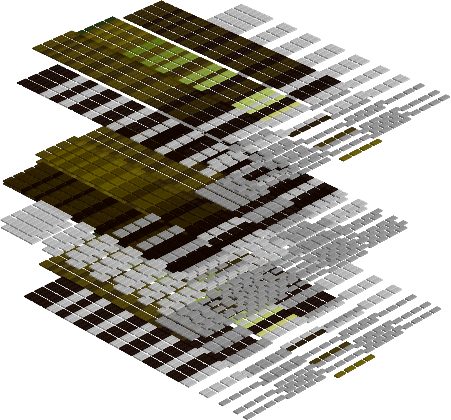
\includegraphics[width=1.5cm]{src/colorspace_colourflow/flows/colourflow_11-45.png}%           
  \end{adjustbox}                                                        
\caption*{

\begin{tikzpicture}                             
\definecolor{tempcolor}{HTML}{000000}           
\fill[tempcolor] (1 mm,0) rectangle ++(1mm,1mm);
\definecolor{tempcolor}{HTML}{bbbbbb}           
\fill[tempcolor] (2 mm,0) rectangle ++(1mm,1mm);
\definecolor{tempcolor}{HTML}{cccccc}           
\fill[tempcolor] (3 mm,0) rectangle ++(1mm,1mm);
\definecolor{tempcolor}{HTML}{eeeeee}           
\fill[tempcolor] (4 mm,0) rectangle ++(1mm,1mm);
\definecolor{tempcolor}{HTML}{190700}           
\fill[tempcolor] (5 mm,0) rectangle ++(1mm,1mm);
\definecolor{tempcolor}{HTML}{3b2900}           
\fill[tempcolor] (6 mm,0) rectangle ++(1mm,1mm);
\definecolor{tempcolor}{HTML}{5d4b00}           
\fill[tempcolor] (7 mm,0) rectangle ++(1mm,1mm);
\definecolor{tempcolor}{HTML}{7f6d00}           
\fill[tempcolor] (8 mm,0) rectangle ++(1mm,1mm);
\end{tikzpicture}                               
}
\end{figure}                                                               
\end{minipage}
\hspace{0.1cm}
\begin{minipage}[b]{0.15\linewidth}
\begin{figure}[H]                                                          
  \centering                                                             
  \begin{adjustbox}{width=1.5cm,center}                                   
  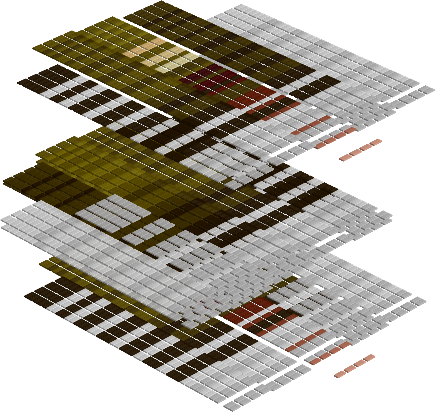
\includegraphics[width=1.5cm]{src/colorspace_colourflow/flows/colourflow_12-45.png}%           
  \end{adjustbox}                                                        
\caption*{

\begin{tikzpicture}                             
\definecolor{tempcolor}{HTML}{000000}           
\fill[tempcolor] (1 mm,0) rectangle ++(1mm,1mm);
\definecolor{tempcolor}{HTML}{cccccc}           
\fill[tempcolor] (2 mm,0) rectangle ++(1mm,1mm);
\definecolor{tempcolor}{HTML}{dddddd}           
\fill[tempcolor] (3 mm,0) rectangle ++(1mm,1mm);
\definecolor{tempcolor}{HTML}{ffffff}           
\fill[tempcolor] (4 mm,0) rectangle ++(1mm,1mm);
\definecolor{tempcolor}{HTML}{2a1800}           
\fill[tempcolor] (5 mm,0) rectangle ++(1mm,1mm);
\definecolor{tempcolor}{HTML}{4c3a00}           
\fill[tempcolor] (6 mm,0) rectangle ++(1mm,1mm);
\definecolor{tempcolor}{HTML}{6e5c00}           
\fill[tempcolor] (7 mm,0) rectangle ++(1mm,1mm);
\definecolor{tempcolor}{HTML}{907e09}           
\fill[tempcolor] (8 mm,0) rectangle ++(1mm,1mm);
\end{tikzpicture}                               
}
\end{figure}                                                               
\end{minipage}
\hspace{0.1cm}
\begin{minipage}[b]{0.15\linewidth}
\begin{figure}[H]                                                          
  \centering                                                             
  \begin{adjustbox}{width=1.5cm,center}                                   
  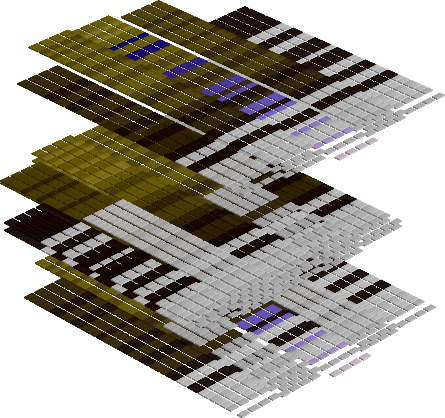
\includegraphics[width=1.5cm]{src/colorspace_colourflow/flows/colourflow_13-45.png}%           
  \end{adjustbox}                                                        
\caption*{

\begin{tikzpicture}                             
\definecolor{tempcolor}{HTML}{000000}           
\fill[tempcolor] (1 mm,0) rectangle ++(1mm,1mm);
\definecolor{tempcolor}{HTML}{dddddd}           
\fill[tempcolor] (2 mm,0) rectangle ++(1mm,1mm);
\definecolor{tempcolor}{HTML}{eeeeee}           
\fill[tempcolor] (3 mm,0) rectangle ++(1mm,1mm);
\definecolor{tempcolor}{HTML}{190700}           
\fill[tempcolor] (4 mm,0) rectangle ++(1mm,1mm);
\definecolor{tempcolor}{HTML}{3b2900}           
\fill[tempcolor] (5 mm,0) rectangle ++(1mm,1mm);
\definecolor{tempcolor}{HTML}{5d4b00}           
\fill[tempcolor] (6 mm,0) rectangle ++(1mm,1mm);
\definecolor{tempcolor}{HTML}{7f6d00}           
\fill[tempcolor] (7 mm,0) rectangle ++(1mm,1mm);
\definecolor{tempcolor}{HTML}{a18f1a}           
\fill[tempcolor] (8 mm,0) rectangle ++(1mm,1mm);
\end{tikzpicture}                               
}
\end{figure}                                                               
\end{minipage}
\hspace{0.1cm}
\begin{minipage}[b]{0.15\linewidth}
\begin{figure}[H]                                                          
  \centering                                                             
  \begin{adjustbox}{width=1.5cm,center}                                   
  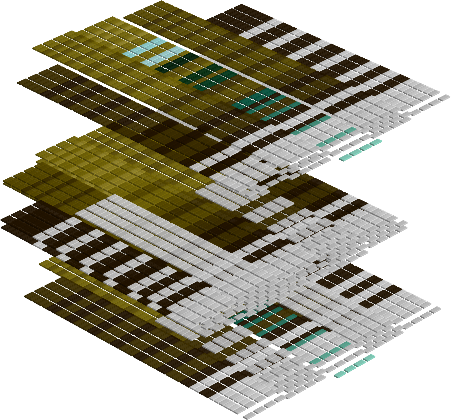
\includegraphics[width=1.5cm]{src/colorspace_colourflow/flows/colourflow_14-45.png}%           
  \end{adjustbox}                                                        
\caption*{

\begin{tikzpicture}                             
\definecolor{tempcolor}{HTML}{000000}           
\fill[tempcolor] (1 mm,0) rectangle ++(1mm,1mm);
\definecolor{tempcolor}{HTML}{eeeeee}           
\fill[tempcolor] (2 mm,0) rectangle ++(1mm,1mm);
\definecolor{tempcolor}{HTML}{ffffff}           
\fill[tempcolor] (3 mm,0) rectangle ++(1mm,1mm);
\definecolor{tempcolor}{HTML}{2a1800}           
\fill[tempcolor] (4 mm,0) rectangle ++(1mm,1mm);
\definecolor{tempcolor}{HTML}{4c3a00}           
\fill[tempcolor] (5 mm,0) rectangle ++(1mm,1mm);
\definecolor{tempcolor}{HTML}{6e5c00}           
\fill[tempcolor] (6 mm,0) rectangle ++(1mm,1mm);
\definecolor{tempcolor}{HTML}{907e09}           
\fill[tempcolor] (7 mm,0) rectangle ++(1mm,1mm);
\definecolor{tempcolor}{HTML}{b3a02b}           
\fill[tempcolor] (8 mm,0) rectangle ++(1mm,1mm);
\end{tikzpicture}                               
}
\end{figure}                                                               
\end{minipage}
\hspace{0.1cm}
\begin{minipage}[b]{0.15\linewidth}
\begin{figure}[H]                                                          
  \centering                                                             
  \begin{adjustbox}{width=1.5cm,center}                                   
  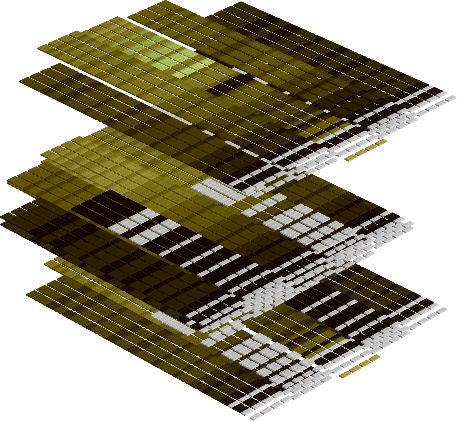
\includegraphics[width=1.5cm]{src/colorspace_colourflow/flows/colourflow_15-45.png}%           
  \end{adjustbox}                                                        
\caption*{

\begin{tikzpicture}                             
\definecolor{tempcolor}{HTML}{000000}           
\fill[tempcolor] (1 mm,0) rectangle ++(1mm,1mm);
\definecolor{tempcolor}{HTML}{ffffff}           
\fill[tempcolor] (2 mm,0) rectangle ++(1mm,1mm);
\definecolor{tempcolor}{HTML}{190700}           
\fill[tempcolor] (3 mm,0) rectangle ++(1mm,1mm);
\definecolor{tempcolor}{HTML}{3b2900}           
\fill[tempcolor] (4 mm,0) rectangle ++(1mm,1mm);
\definecolor{tempcolor}{HTML}{5d4b00}           
\fill[tempcolor] (5 mm,0) rectangle ++(1mm,1mm);
\definecolor{tempcolor}{HTML}{7f6d00}           
\fill[tempcolor] (6 mm,0) rectangle ++(1mm,1mm);
\definecolor{tempcolor}{HTML}{a18f1a}           
\fill[tempcolor] (7 mm,0) rectangle ++(1mm,1mm);
\definecolor{tempcolor}{HTML}{c3b13c}           
\fill[tempcolor] (8 mm,0) rectangle ++(1mm,1mm);
\end{tikzpicture}                               
}
\end{figure}                                                               
\end{minipage}
\hspace{0.1cm}
\begin{minipage}[b]{0.15\linewidth}
\begin{figure}[H]                                                          
  \centering                                                             
  \begin{adjustbox}{width=1.5cm,center}                                   
  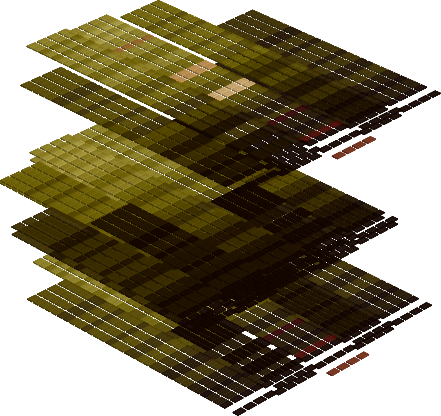
\includegraphics[width=1.5cm]{src/colorspace_colourflow/flows/colourflow_16-45.png}%           
  \end{adjustbox}                                                        
\caption*{

\begin{tikzpicture}                             
\definecolor{tempcolor}{HTML}{000000}           
\fill[tempcolor] (1 mm,0) rectangle ++(1mm,1mm);
\definecolor{tempcolor}{HTML}{190700}           
\fill[tempcolor] (2 mm,0) rectangle ++(1mm,1mm);
\definecolor{tempcolor}{HTML}{2a1800}           
\fill[tempcolor] (3 mm,0) rectangle ++(1mm,1mm);
\definecolor{tempcolor}{HTML}{4c3a00}           
\fill[tempcolor] (4 mm,0) rectangle ++(1mm,1mm);
\definecolor{tempcolor}{HTML}{6e5c00}           
\fill[tempcolor] (5 mm,0) rectangle ++(1mm,1mm);
\definecolor{tempcolor}{HTML}{907e09}           
\fill[tempcolor] (6 mm,0) rectangle ++(1mm,1mm);
\definecolor{tempcolor}{HTML}{b3a02b}           
\fill[tempcolor] (7 mm,0) rectangle ++(1mm,1mm);
\definecolor{tempcolor}{HTML}{d4c24d}           
\fill[tempcolor] (8 mm,0) rectangle ++(1mm,1mm);
\end{tikzpicture}                               
}
\end{figure}                                                               
\end{minipage}
\hspace{0.1cm}
\begin{minipage}[b]{0.15\linewidth}
\begin{figure}[H]                                                          
  \centering                                                             
  \begin{adjustbox}{width=1.5cm,center}                                   
  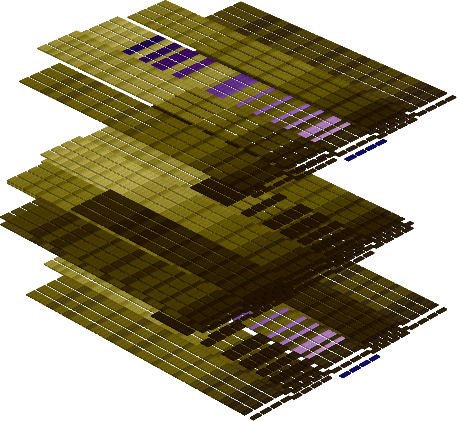
\includegraphics[width=1.5cm]{src/colorspace_colourflow/flows/colourflow_17-45.png}%           
  \end{adjustbox}                                                        
\caption*{

\begin{tikzpicture}                             
\definecolor{tempcolor}{HTML}{000000}           
\fill[tempcolor] (1 mm,0) rectangle ++(1mm,1mm);
\definecolor{tempcolor}{HTML}{2a1800}           
\fill[tempcolor] (2 mm,0) rectangle ++(1mm,1mm);
\definecolor{tempcolor}{HTML}{3b2900}           
\fill[tempcolor] (3 mm,0) rectangle ++(1mm,1mm);
\definecolor{tempcolor}{HTML}{5d4b00}           
\fill[tempcolor] (4 mm,0) rectangle ++(1mm,1mm);
\definecolor{tempcolor}{HTML}{7f6d00}           
\fill[tempcolor] (5 mm,0) rectangle ++(1mm,1mm);
\definecolor{tempcolor}{HTML}{a18f1a}           
\fill[tempcolor] (6 mm,0) rectangle ++(1mm,1mm);
\definecolor{tempcolor}{HTML}{c3b13c}           
\fill[tempcolor] (7 mm,0) rectangle ++(1mm,1mm);
\definecolor{tempcolor}{HTML}{e5d35e}           
\fill[tempcolor] (8 mm,0) rectangle ++(1mm,1mm);
\end{tikzpicture}                               
}
\end{figure}                                                               
\end{minipage}
\hspace{0.1cm}
\begin{minipage}[b]{0.15\linewidth}
\begin{figure}[H]                                                          
  \centering                                                             
  \begin{adjustbox}{width=1.5cm,center}                                   
  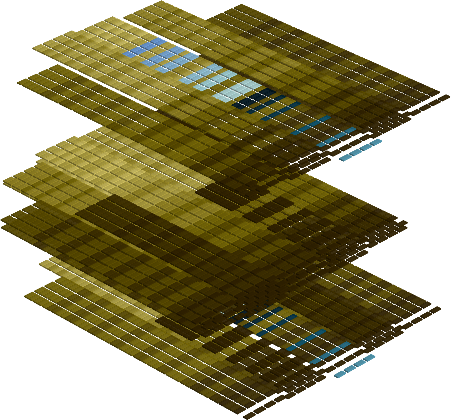
\includegraphics[width=1.5cm]{src/colorspace_colourflow/flows/colourflow_18-45.png}%           
  \end{adjustbox}                                                        
\caption*{

\begin{tikzpicture}                             
\definecolor{tempcolor}{HTML}{000000}           
\fill[tempcolor] (1 mm,0) rectangle ++(1mm,1mm);
\definecolor{tempcolor}{HTML}{3b2900}           
\fill[tempcolor] (2 mm,0) rectangle ++(1mm,1mm);
\definecolor{tempcolor}{HTML}{4c3a00}           
\fill[tempcolor] (3 mm,0) rectangle ++(1mm,1mm);
\definecolor{tempcolor}{HTML}{6e5c00}           
\fill[tempcolor] (4 mm,0) rectangle ++(1mm,1mm);
\definecolor{tempcolor}{HTML}{907e09}           
\fill[tempcolor] (5 mm,0) rectangle ++(1mm,1mm);
\definecolor{tempcolor}{HTML}{b3a02b}           
\fill[tempcolor] (6 mm,0) rectangle ++(1mm,1mm);
\definecolor{tempcolor}{HTML}{d4c24d}           
\fill[tempcolor] (7 mm,0) rectangle ++(1mm,1mm);
\definecolor{tempcolor}{HTML}{f7e46f}           
\fill[tempcolor] (8 mm,0) rectangle ++(1mm,1mm);
\end{tikzpicture}                               
}
\end{figure}                                                               
\end{minipage}
\hspace{0.1cm}
\begin{minipage}[b]{0.15\linewidth}
\begin{figure}[H]                                                          
  \centering                                                             
  \begin{adjustbox}{width=1.5cm,center}                                   
  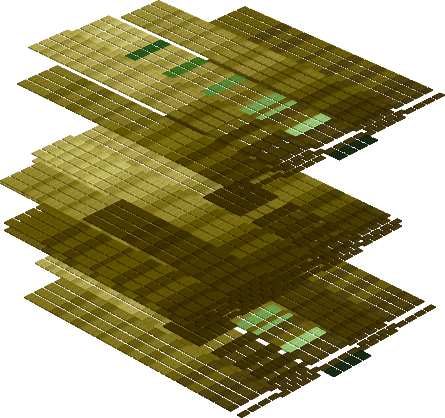
\includegraphics[width=1.5cm]{src/colorspace_colourflow/flows/colourflow_19-45.png}%           
  \end{adjustbox}                                                        
\caption*{

\begin{tikzpicture}                             
\definecolor{tempcolor}{HTML}{000000}           
\fill[tempcolor] (1 mm,0) rectangle ++(1mm,1mm);
\definecolor{tempcolor}{HTML}{4c3a00}           
\fill[tempcolor] (2 mm,0) rectangle ++(1mm,1mm);
\definecolor{tempcolor}{HTML}{5d4b00}           
\fill[tempcolor] (3 mm,0) rectangle ++(1mm,1mm);
\definecolor{tempcolor}{HTML}{7f6d00}           
\fill[tempcolor] (4 mm,0) rectangle ++(1mm,1mm);
\definecolor{tempcolor}{HTML}{a18f1a}           
\fill[tempcolor] (5 mm,0) rectangle ++(1mm,1mm);
\definecolor{tempcolor}{HTML}{c3b13c}           
\fill[tempcolor] (6 mm,0) rectangle ++(1mm,1mm);
\definecolor{tempcolor}{HTML}{e5d35e}           
\fill[tempcolor] (7 mm,0) rectangle ++(1mm,1mm);
\definecolor{tempcolor}{HTML}{fff582}           
\fill[tempcolor] (8 mm,0) rectangle ++(1mm,1mm);
\end{tikzpicture}                               
}
\end{figure}                                                               
\end{minipage}
\hspace{0.1cm}
\begin{minipage}[b]{0.15\linewidth}
\begin{figure}[H]                                                          
  \centering                                                             
  \begin{adjustbox}{width=1.5cm,center}                                   
  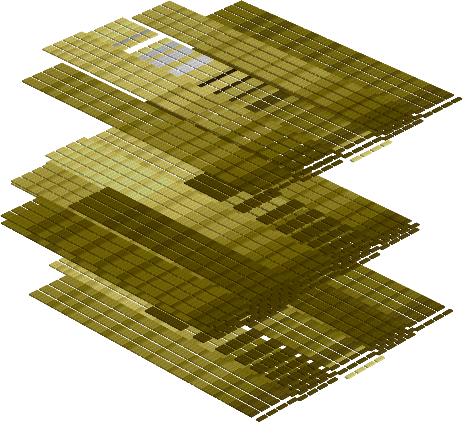
\includegraphics[width=1.5cm]{src/colorspace_colourflow/flows/colourflow_20-45.png}%           
  \end{adjustbox}                                                        
\caption*{

\begin{tikzpicture}                             
\definecolor{tempcolor}{HTML}{000000}           
\fill[tempcolor] (1 mm,0) rectangle ++(1mm,1mm);
\definecolor{tempcolor}{HTML}{5d4b00}           
\fill[tempcolor] (2 mm,0) rectangle ++(1mm,1mm);
\definecolor{tempcolor}{HTML}{6e5c00}           
\fill[tempcolor] (3 mm,0) rectangle ++(1mm,1mm);
\definecolor{tempcolor}{HTML}{907e09}           
\fill[tempcolor] (4 mm,0) rectangle ++(1mm,1mm);
\definecolor{tempcolor}{HTML}{b3a02b}           
\fill[tempcolor] (5 mm,0) rectangle ++(1mm,1mm);
\definecolor{tempcolor}{HTML}{d4c24d}           
\fill[tempcolor] (6 mm,0) rectangle ++(1mm,1mm);
\definecolor{tempcolor}{HTML}{f7e46f}           
\fill[tempcolor] (7 mm,0) rectangle ++(1mm,1mm);
\definecolor{tempcolor}{HTML}{ffff96}           
\fill[tempcolor] (8 mm,0) rectangle ++(1mm,1mm);
\end{tikzpicture}                               
}
\end{figure}                                                               
\end{minipage}
\hspace{0.1cm}
\begin{minipage}[b]{0.15\linewidth}
\begin{figure}[H]                                                          
  \centering                                                             
  \begin{adjustbox}{width=1.5cm,center}                                   
  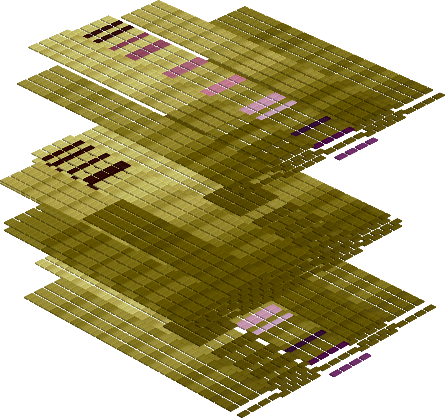
\includegraphics[width=1.5cm]{src/colorspace_colourflow/flows/colourflow_21-45.png}%           
  \end{adjustbox}                                                        
\caption*{

\begin{tikzpicture}                             
\definecolor{tempcolor}{HTML}{000000}           
\fill[tempcolor] (1 mm,0) rectangle ++(1mm,1mm);
\definecolor{tempcolor}{HTML}{6e5c00}           
\fill[tempcolor] (2 mm,0) rectangle ++(1mm,1mm);
\definecolor{tempcolor}{HTML}{7f6d00}           
\fill[tempcolor] (3 mm,0) rectangle ++(1mm,1mm);
\definecolor{tempcolor}{HTML}{a18f1a}           
\fill[tempcolor] (4 mm,0) rectangle ++(1mm,1mm);
\definecolor{tempcolor}{HTML}{c3b13c}           
\fill[tempcolor] (5 mm,0) rectangle ++(1mm,1mm);
\definecolor{tempcolor}{HTML}{e5d35e}           
\fill[tempcolor] (6 mm,0) rectangle ++(1mm,1mm);
\definecolor{tempcolor}{HTML}{fff582}           
\fill[tempcolor] (7 mm,0) rectangle ++(1mm,1mm);
\definecolor{tempcolor}{HTML}{310000}           
\fill[tempcolor] (8 mm,0) rectangle ++(1mm,1mm);
\end{tikzpicture}                               
}
\end{figure}                                                               
\end{minipage}
\hspace{0.1cm}
\begin{minipage}[b]{0.15\linewidth}
\begin{figure}[H]                                                          
  \centering                                                             
  \begin{adjustbox}{width=1.5cm,center}                                   
  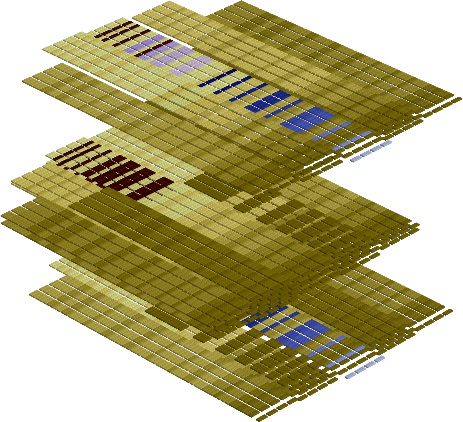
\includegraphics[width=1.5cm]{src/colorspace_colourflow/flows/colourflow_22-45.png}%           
  \end{adjustbox}                                                        
\caption*{

\begin{tikzpicture}                             
\definecolor{tempcolor}{HTML}{000000}           
\fill[tempcolor] (1 mm,0) rectangle ++(1mm,1mm);
\definecolor{tempcolor}{HTML}{7f6d00}           
\fill[tempcolor] (2 mm,0) rectangle ++(1mm,1mm);
\definecolor{tempcolor}{HTML}{907e09}           
\fill[tempcolor] (3 mm,0) rectangle ++(1mm,1mm);
\definecolor{tempcolor}{HTML}{b3a02b}           
\fill[tempcolor] (4 mm,0) rectangle ++(1mm,1mm);
\definecolor{tempcolor}{HTML}{d4c24d}           
\fill[tempcolor] (5 mm,0) rectangle ++(1mm,1mm);
\definecolor{tempcolor}{HTML}{f7e46f}           
\fill[tempcolor] (6 mm,0) rectangle ++(1mm,1mm);
\definecolor{tempcolor}{HTML}{ffff96}           
\fill[tempcolor] (7 mm,0) rectangle ++(1mm,1mm);
\definecolor{tempcolor}{HTML}{3f0000}           
\fill[tempcolor] (8 mm,0) rectangle ++(1mm,1mm);
\end{tikzpicture}                               
}
\end{figure}                                                               
\end{minipage}
\hspace{0.1cm}
\begin{minipage}[b]{0.15\linewidth}
\begin{figure}[H]                                                          
  \centering                                                             
  \begin{adjustbox}{width=1.5cm,center}                                   
  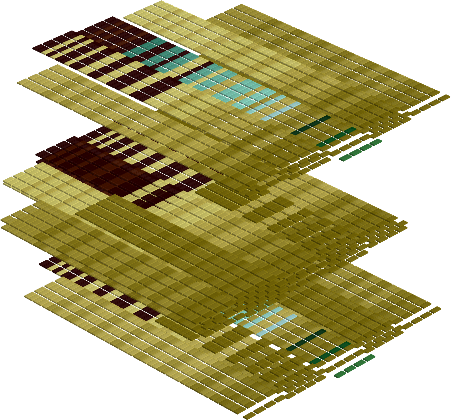
\includegraphics[width=1.5cm]{src/colorspace_colourflow/flows/colourflow_23-45.png}%           
  \end{adjustbox}                                                        
\caption*{

\begin{tikzpicture}                             
\definecolor{tempcolor}{HTML}{000000}           
\fill[tempcolor] (1 mm,0) rectangle ++(1mm,1mm);
\definecolor{tempcolor}{HTML}{907e09}           
\fill[tempcolor] (2 mm,0) rectangle ++(1mm,1mm);
\definecolor{tempcolor}{HTML}{a18f1a}           
\fill[tempcolor] (3 mm,0) rectangle ++(1mm,1mm);
\definecolor{tempcolor}{HTML}{c3b13c}           
\fill[tempcolor] (4 mm,0) rectangle ++(1mm,1mm);
\definecolor{tempcolor}{HTML}{e5d35e}           
\fill[tempcolor] (5 mm,0) rectangle ++(1mm,1mm);
\definecolor{tempcolor}{HTML}{fff582}           
\fill[tempcolor] (6 mm,0) rectangle ++(1mm,1mm);
\definecolor{tempcolor}{HTML}{310000}           
\fill[tempcolor] (7 mm,0) rectangle ++(1mm,1mm);
\definecolor{tempcolor}{HTML}{531700}           
\fill[tempcolor] (8 mm,0) rectangle ++(1mm,1mm);
\end{tikzpicture}                               
}
\end{figure}                                                               
\end{minipage}
\hspace{0.1cm}
\begin{minipage}[b]{0.15\linewidth}
\begin{figure}[H]                                                          
  \centering                                                             
  \begin{adjustbox}{width=1.5cm,center}                                   
  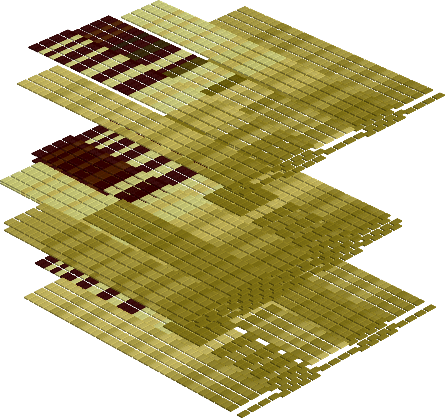
\includegraphics[width=1.5cm]{src/colorspace_colourflow/flows/colourflow_24-45.png}%           
  \end{adjustbox}                                                        
\caption*{

\begin{tikzpicture}                             
\definecolor{tempcolor}{HTML}{000000}           
\fill[tempcolor] (1 mm,0) rectangle ++(1mm,1mm);
\definecolor{tempcolor}{HTML}{a18f1a}           
\fill[tempcolor] (2 mm,0) rectangle ++(1mm,1mm);
\definecolor{tempcolor}{HTML}{b3a02b}           
\fill[tempcolor] (3 mm,0) rectangle ++(1mm,1mm);
\definecolor{tempcolor}{HTML}{d4c24d}           
\fill[tempcolor] (4 mm,0) rectangle ++(1mm,1mm);
\definecolor{tempcolor}{HTML}{f7e46f}           
\fill[tempcolor] (5 mm,0) rectangle ++(1mm,1mm);
\definecolor{tempcolor}{HTML}{ffff96}           
\fill[tempcolor] (6 mm,0) rectangle ++(1mm,1mm);
\definecolor{tempcolor}{HTML}{3f0000}           
\fill[tempcolor] (7 mm,0) rectangle ++(1mm,1mm);
\definecolor{tempcolor}{HTML}{642800}           
\fill[tempcolor] (8 mm,0) rectangle ++(1mm,1mm);
\end{tikzpicture}                               
}
\end{figure}                                                               
\end{minipage}
\hspace{0.1cm}
\begin{minipage}[b]{0.15\linewidth}
\begin{figure}[H]                                                          
  \centering                                                             
  \begin{adjustbox}{width=1.5cm,center}                                   
  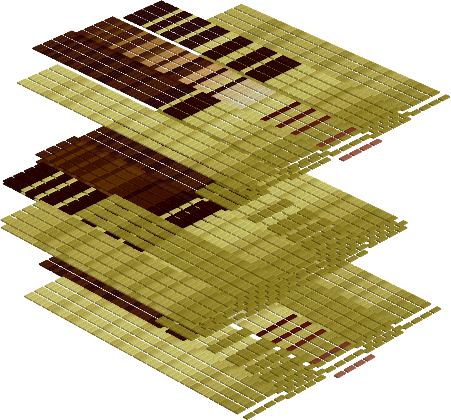
\includegraphics[width=1.5cm]{src/colorspace_colourflow/flows/colourflow_25-45.png}%           
  \end{adjustbox}                                                        
\caption*{

\begin{tikzpicture}                             
\definecolor{tempcolor}{HTML}{000000}           
\fill[tempcolor] (1 mm,0) rectangle ++(1mm,1mm);
\definecolor{tempcolor}{HTML}{b3a02b}           
\fill[tempcolor] (2 mm,0) rectangle ++(1mm,1mm);
\definecolor{tempcolor}{HTML}{c3b13c}           
\fill[tempcolor] (3 mm,0) rectangle ++(1mm,1mm);
\definecolor{tempcolor}{HTML}{e5d35e}           
\fill[tempcolor] (4 mm,0) rectangle ++(1mm,1mm);
\definecolor{tempcolor}{HTML}{fff582}           
\fill[tempcolor] (5 mm,0) rectangle ++(1mm,1mm);
\definecolor{tempcolor}{HTML}{310000}           
\fill[tempcolor] (6 mm,0) rectangle ++(1mm,1mm);
\definecolor{tempcolor}{HTML}{531700}           
\fill[tempcolor] (7 mm,0) rectangle ++(1mm,1mm);
\definecolor{tempcolor}{HTML}{753900}           
\fill[tempcolor] (8 mm,0) rectangle ++(1mm,1mm);
\end{tikzpicture}                               
}
\end{figure}                                                               
\end{minipage}
\hspace{0.1cm}
\begin{minipage}[b]{0.15\linewidth}
\begin{figure}[H]                                                          
  \centering                                                             
  \begin{adjustbox}{width=1.5cm,center}                                   
  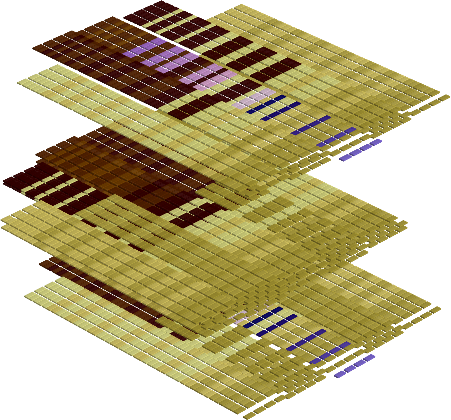
\includegraphics[width=1.5cm]{src/colorspace_colourflow/flows/colourflow_26-45.png}%           
  \end{adjustbox}                                                        
\caption*{

\begin{tikzpicture}                             
\definecolor{tempcolor}{HTML}{000000}           
\fill[tempcolor] (1 mm,0) rectangle ++(1mm,1mm);
\definecolor{tempcolor}{HTML}{c3b13c}           
\fill[tempcolor] (2 mm,0) rectangle ++(1mm,1mm);
\definecolor{tempcolor}{HTML}{d4c24d}           
\fill[tempcolor] (3 mm,0) rectangle ++(1mm,1mm);
\definecolor{tempcolor}{HTML}{f7e46f}           
\fill[tempcolor] (4 mm,0) rectangle ++(1mm,1mm);
\definecolor{tempcolor}{HTML}{ffff96}           
\fill[tempcolor] (5 mm,0) rectangle ++(1mm,1mm);
\definecolor{tempcolor}{HTML}{3f0000}           
\fill[tempcolor] (6 mm,0) rectangle ++(1mm,1mm);
\definecolor{tempcolor}{HTML}{642800}           
\fill[tempcolor] (7 mm,0) rectangle ++(1mm,1mm);
\definecolor{tempcolor}{HTML}{864a00}           
\fill[tempcolor] (8 mm,0) rectangle ++(1mm,1mm);
\end{tikzpicture}                               
}
\end{figure}                                                               
\end{minipage}
\hspace{0.1cm}
\begin{minipage}[b]{0.15\linewidth}
\begin{figure}[H]                                                          
  \centering                                                             
  \begin{adjustbox}{width=1.5cm,center}                                   
  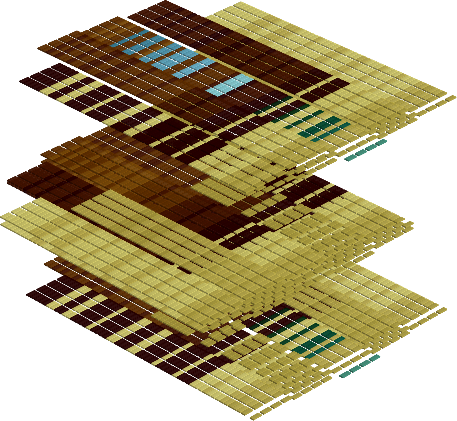
\includegraphics[width=1.5cm]{src/colorspace_colourflow/flows/colourflow_27-45.png}%           
  \end{adjustbox}                                                        
\caption*{

\begin{tikzpicture}                             
\definecolor{tempcolor}{HTML}{000000}           
\fill[tempcolor] (1 mm,0) rectangle ++(1mm,1mm);
\definecolor{tempcolor}{HTML}{d4c24d}           
\fill[tempcolor] (2 mm,0) rectangle ++(1mm,1mm);
\definecolor{tempcolor}{HTML}{e5d35e}           
\fill[tempcolor] (3 mm,0) rectangle ++(1mm,1mm);
\definecolor{tempcolor}{HTML}{fff582}           
\fill[tempcolor] (4 mm,0) rectangle ++(1mm,1mm);
\definecolor{tempcolor}{HTML}{310000}           
\fill[tempcolor] (5 mm,0) rectangle ++(1mm,1mm);
\definecolor{tempcolor}{HTML}{531700}           
\fill[tempcolor] (6 mm,0) rectangle ++(1mm,1mm);
\definecolor{tempcolor}{HTML}{753900}           
\fill[tempcolor] (7 mm,0) rectangle ++(1mm,1mm);
\definecolor{tempcolor}{HTML}{975b0a}           
\fill[tempcolor] (8 mm,0) rectangle ++(1mm,1mm);
\end{tikzpicture}                               
}
\end{figure}                                                               
\end{minipage}
\hspace{0.1cm}
\begin{minipage}[b]{0.15\linewidth}
\begin{figure}[H]                                                          
  \centering                                                             
  \begin{adjustbox}{width=1.5cm,center}                                   
  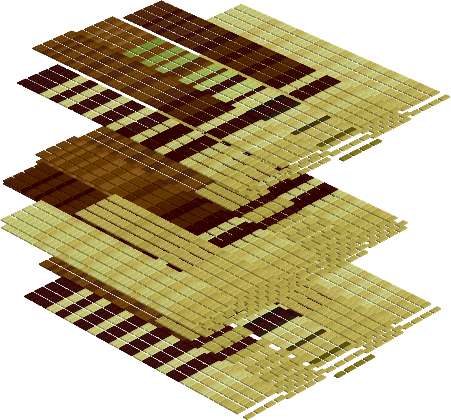
\includegraphics[width=1.5cm]{src/colorspace_colourflow/flows/colourflow_28-45.png}%           
  \end{adjustbox}                                                        
\caption*{

\begin{tikzpicture}                             
\definecolor{tempcolor}{HTML}{000000}           
\fill[tempcolor] (1 mm,0) rectangle ++(1mm,1mm);
\definecolor{tempcolor}{HTML}{e5d35e}           
\fill[tempcolor] (2 mm,0) rectangle ++(1mm,1mm);
\definecolor{tempcolor}{HTML}{f7e46f}           
\fill[tempcolor] (3 mm,0) rectangle ++(1mm,1mm);
\definecolor{tempcolor}{HTML}{ffff96}           
\fill[tempcolor] (4 mm,0) rectangle ++(1mm,1mm);
\definecolor{tempcolor}{HTML}{3f0000}           
\fill[tempcolor] (5 mm,0) rectangle ++(1mm,1mm);
\definecolor{tempcolor}{HTML}{642800}           
\fill[tempcolor] (6 mm,0) rectangle ++(1mm,1mm);
\definecolor{tempcolor}{HTML}{864a00}           
\fill[tempcolor] (7 mm,0) rectangle ++(1mm,1mm);
\definecolor{tempcolor}{HTML}{a86c1b}           
\fill[tempcolor] (8 mm,0) rectangle ++(1mm,1mm);
\end{tikzpicture}                               
}
\end{figure}                                                               
\end{minipage}
\hspace{0.1cm}
\begin{minipage}[b]{0.15\linewidth}
\begin{figure}[H]                                                          
  \centering                                                             
  \begin{adjustbox}{width=1.5cm,center}                                   
  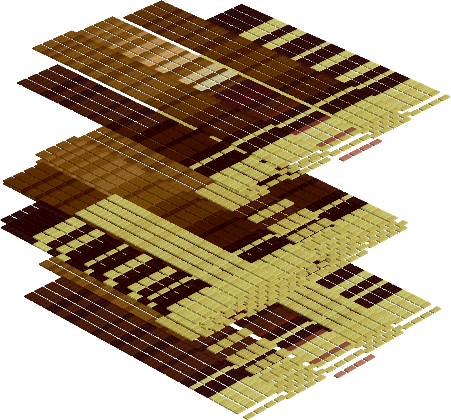
\includegraphics[width=1.5cm]{src/colorspace_colourflow/flows/colourflow_29-45.png}%           
  \end{adjustbox}                                                        
\caption*{

\begin{tikzpicture}                             
\definecolor{tempcolor}{HTML}{000000}           
\fill[tempcolor] (1 mm,0) rectangle ++(1mm,1mm);
\definecolor{tempcolor}{HTML}{f7e46f}           
\fill[tempcolor] (2 mm,0) rectangle ++(1mm,1mm);
\definecolor{tempcolor}{HTML}{fff582}           
\fill[tempcolor] (3 mm,0) rectangle ++(1mm,1mm);
\definecolor{tempcolor}{HTML}{310000}           
\fill[tempcolor] (4 mm,0) rectangle ++(1mm,1mm);
\definecolor{tempcolor}{HTML}{531700}           
\fill[tempcolor] (5 mm,0) rectangle ++(1mm,1mm);
\definecolor{tempcolor}{HTML}{753900}           
\fill[tempcolor] (6 mm,0) rectangle ++(1mm,1mm);
\definecolor{tempcolor}{HTML}{975b0a}           
\fill[tempcolor] (7 mm,0) rectangle ++(1mm,1mm);
\definecolor{tempcolor}{HTML}{b97d2c}           
\fill[tempcolor] (8 mm,0) rectangle ++(1mm,1mm);
\end{tikzpicture}                               
}
\end{figure}                                                               
\end{minipage}
\hspace{0.1cm}
\begin{minipage}[b]{0.15\linewidth}
\begin{figure}[H]                                                          
  \centering                                                             
  \begin{adjustbox}{width=1.5cm,center}                                   
  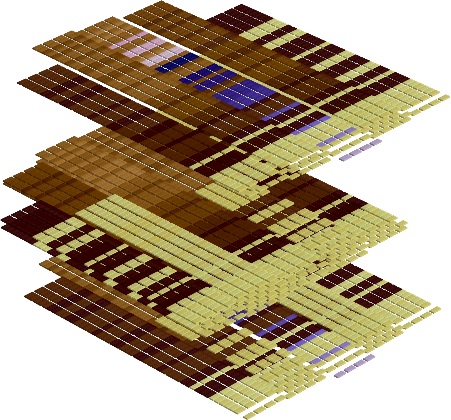
\includegraphics[width=1.5cm]{src/colorspace_colourflow/flows/colourflow_30-45.png}%           
  \end{adjustbox}                                                        
\caption*{

\begin{tikzpicture}                             
\definecolor{tempcolor}{HTML}{000000}           
\fill[tempcolor] (1 mm,0) rectangle ++(1mm,1mm);
\definecolor{tempcolor}{HTML}{fff582}           
\fill[tempcolor] (2 mm,0) rectangle ++(1mm,1mm);
\definecolor{tempcolor}{HTML}{ffff96}           
\fill[tempcolor] (3 mm,0) rectangle ++(1mm,1mm);
\definecolor{tempcolor}{HTML}{3f0000}           
\fill[tempcolor] (4 mm,0) rectangle ++(1mm,1mm);
\definecolor{tempcolor}{HTML}{642800}           
\fill[tempcolor] (5 mm,0) rectangle ++(1mm,1mm);
\definecolor{tempcolor}{HTML}{864a00}           
\fill[tempcolor] (6 mm,0) rectangle ++(1mm,1mm);
\definecolor{tempcolor}{HTML}{a86c1b}           
\fill[tempcolor] (7 mm,0) rectangle ++(1mm,1mm);
\definecolor{tempcolor}{HTML}{ca8e3d}           
\fill[tempcolor] (8 mm,0) rectangle ++(1mm,1mm);
\end{tikzpicture}                               
}
\end{figure}                                                               
\end{minipage}
\hspace{0.1cm}
\begin{minipage}[b]{0.15\linewidth}
\begin{figure}[H]                                                          
  \centering                                                             
  \begin{adjustbox}{width=1.5cm,center}                                   
  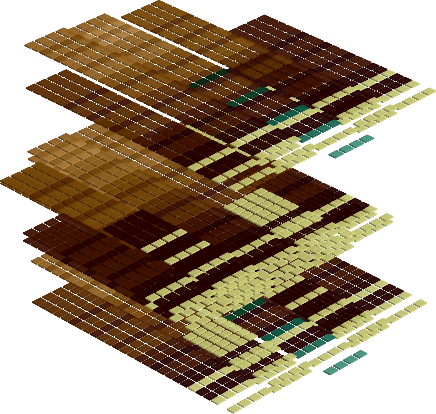
\includegraphics[width=1.5cm]{src/colorspace_colourflow/flows/colourflow_31-45.png}%           
  \end{adjustbox}                                                        
\caption*{

\begin{tikzpicture}                             
\definecolor{tempcolor}{HTML}{000000}           
\fill[tempcolor] (1 mm,0) rectangle ++(1mm,1mm);
\definecolor{tempcolor}{HTML}{ffff96}           
\fill[tempcolor] (2 mm,0) rectangle ++(1mm,1mm);
\definecolor{tempcolor}{HTML}{310000}           
\fill[tempcolor] (3 mm,0) rectangle ++(1mm,1mm);
\definecolor{tempcolor}{HTML}{531700}           
\fill[tempcolor] (4 mm,0) rectangle ++(1mm,1mm);
\definecolor{tempcolor}{HTML}{753900}           
\fill[tempcolor] (5 mm,0) rectangle ++(1mm,1mm);
\definecolor{tempcolor}{HTML}{975b0a}           
\fill[tempcolor] (6 mm,0) rectangle ++(1mm,1mm);
\definecolor{tempcolor}{HTML}{b97d2c}           
\fill[tempcolor] (7 mm,0) rectangle ++(1mm,1mm);
\definecolor{tempcolor}{HTML}{db9f4e}           
\fill[tempcolor] (8 mm,0) rectangle ++(1mm,1mm);
\end{tikzpicture}                               
}
\end{figure}                                                               
\end{minipage}
\hspace{0.1cm}
\begin{minipage}[b]{0.15\linewidth}
\begin{figure}[H]                                                          
  \centering                                                             
  \begin{adjustbox}{width=1.5cm,center}                                   
  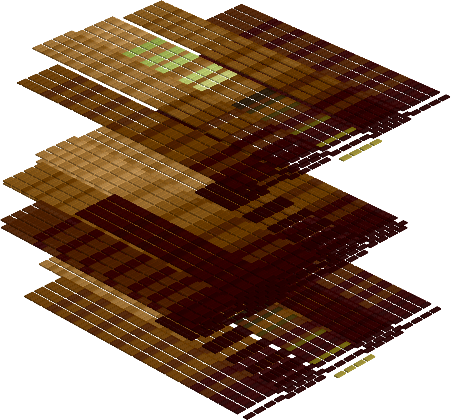
\includegraphics[width=1.5cm]{src/colorspace_colourflow/flows/colourflow_32-45.png}%           
  \end{adjustbox}                                                        
\caption*{

\begin{tikzpicture}                             
\definecolor{tempcolor}{HTML}{000000}           
\fill[tempcolor] (1 mm,0) rectangle ++(1mm,1mm);
\definecolor{tempcolor}{HTML}{310000}           
\fill[tempcolor] (2 mm,0) rectangle ++(1mm,1mm);
\definecolor{tempcolor}{HTML}{3f0000}           
\fill[tempcolor] (3 mm,0) rectangle ++(1mm,1mm);
\definecolor{tempcolor}{HTML}{642800}           
\fill[tempcolor] (4 mm,0) rectangle ++(1mm,1mm);
\definecolor{tempcolor}{HTML}{864a00}           
\fill[tempcolor] (5 mm,0) rectangle ++(1mm,1mm);
\definecolor{tempcolor}{HTML}{a86c1b}           
\fill[tempcolor] (6 mm,0) rectangle ++(1mm,1mm);
\definecolor{tempcolor}{HTML}{ca8e3d}           
\fill[tempcolor] (7 mm,0) rectangle ++(1mm,1mm);
\definecolor{tempcolor}{HTML}{ecb05f}           
\fill[tempcolor] (8 mm,0) rectangle ++(1mm,1mm);
\end{tikzpicture}                               
}
\end{figure}                                                               
\end{minipage}
\hspace{0.1cm}
\begin{minipage}[b]{0.15\linewidth}
\begin{figure}[H]                                                          
  \centering                                                             
  \begin{adjustbox}{width=1.5cm,center}                                   
  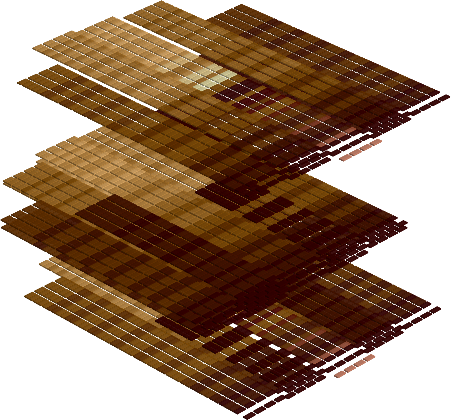
\includegraphics[width=1.5cm]{src/colorspace_colourflow/flows/colourflow_33-45.png}%           
  \end{adjustbox}                                                        
\caption*{

\begin{tikzpicture}                             
\definecolor{tempcolor}{HTML}{000000}           
\fill[tempcolor] (1 mm,0) rectangle ++(1mm,1mm);
\definecolor{tempcolor}{HTML}{3f0000}           
\fill[tempcolor] (2 mm,0) rectangle ++(1mm,1mm);
\definecolor{tempcolor}{HTML}{531700}           
\fill[tempcolor] (3 mm,0) rectangle ++(1mm,1mm);
\definecolor{tempcolor}{HTML}{753900}           
\fill[tempcolor] (4 mm,0) rectangle ++(1mm,1mm);
\definecolor{tempcolor}{HTML}{975b0a}           
\fill[tempcolor] (5 mm,0) rectangle ++(1mm,1mm);
\definecolor{tempcolor}{HTML}{b97d2c}           
\fill[tempcolor] (6 mm,0) rectangle ++(1mm,1mm);
\definecolor{tempcolor}{HTML}{db9f4e}           
\fill[tempcolor] (7 mm,0) rectangle ++(1mm,1mm);
\definecolor{tempcolor}{HTML}{fdc170}           
\fill[tempcolor] (8 mm,0) rectangle ++(1mm,1mm);
\end{tikzpicture}                               
}
\end{figure}                                                               
\end{minipage}
\hspace{0.1cm}
\begin{minipage}[b]{0.15\linewidth}
\begin{figure}[H]                                                          
  \centering                                                             
  \begin{adjustbox}{width=1.5cm,center}                                   
  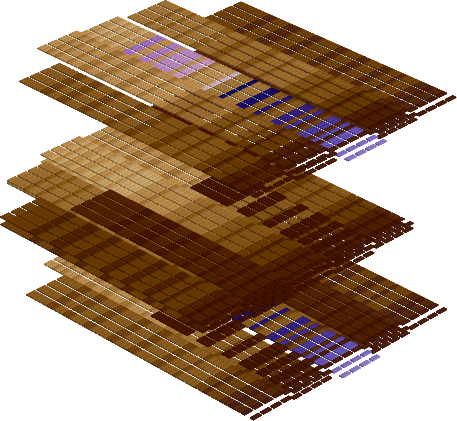
\includegraphics[width=1.5cm]{src/colorspace_colourflow/flows/colourflow_34-45.png}%           
  \end{adjustbox}                                                        
\caption*{

\begin{tikzpicture}                             
\definecolor{tempcolor}{HTML}{000000}           
\fill[tempcolor] (1 mm,0) rectangle ++(1mm,1mm);
\definecolor{tempcolor}{HTML}{531700}           
\fill[tempcolor] (2 mm,0) rectangle ++(1mm,1mm);
\definecolor{tempcolor}{HTML}{642800}           
\fill[tempcolor] (3 mm,0) rectangle ++(1mm,1mm);
\definecolor{tempcolor}{HTML}{864a00}           
\fill[tempcolor] (4 mm,0) rectangle ++(1mm,1mm);
\definecolor{tempcolor}{HTML}{a86c1b}           
\fill[tempcolor] (5 mm,0) rectangle ++(1mm,1mm);
\definecolor{tempcolor}{HTML}{ca8e3d}           
\fill[tempcolor] (6 mm,0) rectangle ++(1mm,1mm);
\definecolor{tempcolor}{HTML}{ecb05f}           
\fill[tempcolor] (7 mm,0) rectangle ++(1mm,1mm);
\definecolor{tempcolor}{HTML}{ffd285}           
\fill[tempcolor] (8 mm,0) rectangle ++(1mm,1mm);
\end{tikzpicture}                               
}
\end{figure}                                                               
\end{minipage}
\hspace{0.1cm}
\begin{minipage}[b]{0.15\linewidth}
\begin{figure}[H]                                                          
  \centering                                                             
  \begin{adjustbox}{width=1.5cm,center}                                   
  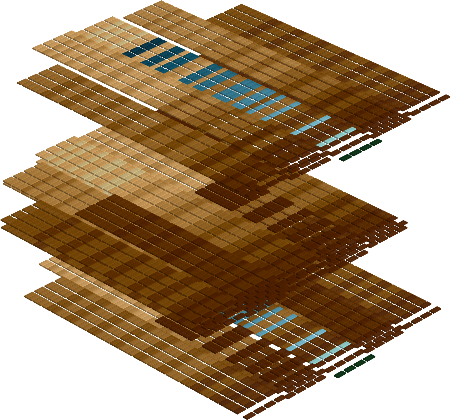
\includegraphics[width=1.5cm]{src/colorspace_colourflow/flows/colourflow_35-45.png}%           
  \end{adjustbox}                                                        
\caption*{

\begin{tikzpicture}                             
\definecolor{tempcolor}{HTML}{000000}           
\fill[tempcolor] (1 mm,0) rectangle ++(1mm,1mm);
\definecolor{tempcolor}{HTML}{642800}           
\fill[tempcolor] (2 mm,0) rectangle ++(1mm,1mm);
\definecolor{tempcolor}{HTML}{753900}           
\fill[tempcolor] (3 mm,0) rectangle ++(1mm,1mm);
\definecolor{tempcolor}{HTML}{975b0a}           
\fill[tempcolor] (4 mm,0) rectangle ++(1mm,1mm);
\definecolor{tempcolor}{HTML}{b97d2c}           
\fill[tempcolor] (5 mm,0) rectangle ++(1mm,1mm);
\definecolor{tempcolor}{HTML}{db9f4e}           
\fill[tempcolor] (6 mm,0) rectangle ++(1mm,1mm);
\definecolor{tempcolor}{HTML}{fdc170}           
\fill[tempcolor] (7 mm,0) rectangle ++(1mm,1mm);
\definecolor{tempcolor}{HTML}{ffe39c}           
\fill[tempcolor] (8 mm,0) rectangle ++(1mm,1mm);
\end{tikzpicture}                               
}
\end{figure}                                                               
\end{minipage}
\hspace{0.1cm}
\begin{minipage}[b]{0.15\linewidth}
\begin{figure}[H]                                                          
  \centering                                                             
  \begin{adjustbox}{width=1.5cm,center}                                   
  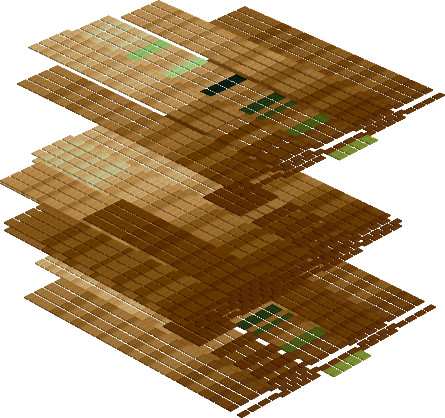
\includegraphics[width=1.5cm]{src/colorspace_colourflow/flows/colourflow_36-45.png}%           
  \end{adjustbox}                                                        
\caption*{

\begin{tikzpicture}                             
\definecolor{tempcolor}{HTML}{000000}           
\fill[tempcolor] (1 mm,0) rectangle ++(1mm,1mm);
\definecolor{tempcolor}{HTML}{753900}           
\fill[tempcolor] (2 mm,0) rectangle ++(1mm,1mm);
\definecolor{tempcolor}{HTML}{864a00}           
\fill[tempcolor] (3 mm,0) rectangle ++(1mm,1mm);
\definecolor{tempcolor}{HTML}{a86c1b}           
\fill[tempcolor] (4 mm,0) rectangle ++(1mm,1mm);
\definecolor{tempcolor}{HTML}{ca8e3d}           
\fill[tempcolor] (5 mm,0) rectangle ++(1mm,1mm);
\definecolor{tempcolor}{HTML}{ecb05f}           
\fill[tempcolor] (6 mm,0) rectangle ++(1mm,1mm);
\definecolor{tempcolor}{HTML}{ffd285}           
\fill[tempcolor] (7 mm,0) rectangle ++(1mm,1mm);
\definecolor{tempcolor}{HTML}{fff4b2}           
\fill[tempcolor] (8 mm,0) rectangle ++(1mm,1mm);
\end{tikzpicture}                               
}
\end{figure}                                                               
\end{minipage}
\hspace{0.1cm}
\begin{minipage}[b]{0.15\linewidth}
\begin{figure}[H]                                                          
  \centering                                                             
  \begin{adjustbox}{width=1.5cm,center}                                   
  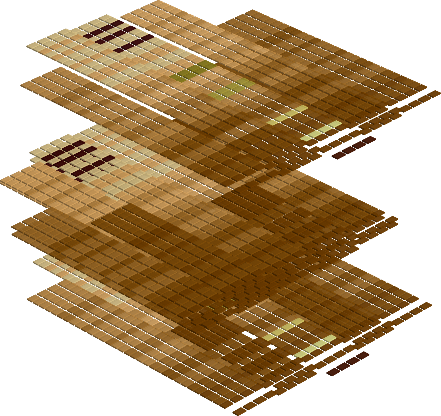
\includegraphics[width=1.5cm]{src/colorspace_colourflow/flows/colourflow_37-45.png}%           
  \end{adjustbox}                                                        
\caption*{

\begin{tikzpicture}                             
\definecolor{tempcolor}{HTML}{000000}           
\fill[tempcolor] (1 mm,0) rectangle ++(1mm,1mm);
\definecolor{tempcolor}{HTML}{864a00}           
\fill[tempcolor] (2 mm,0) rectangle ++(1mm,1mm);
\definecolor{tempcolor}{HTML}{975b0a}           
\fill[tempcolor] (3 mm,0) rectangle ++(1mm,1mm);
\definecolor{tempcolor}{HTML}{b97d2c}           
\fill[tempcolor] (4 mm,0) rectangle ++(1mm,1mm);
\definecolor{tempcolor}{HTML}{db9f4e}           
\fill[tempcolor] (5 mm,0) rectangle ++(1mm,1mm);
\definecolor{tempcolor}{HTML}{fdc170}           
\fill[tempcolor] (6 mm,0) rectangle ++(1mm,1mm);
\definecolor{tempcolor}{HTML}{ffe39c}           
\fill[tempcolor] (7 mm,0) rectangle ++(1mm,1mm);
\definecolor{tempcolor}{HTML}{420404}           
\fill[tempcolor] (8 mm,0) rectangle ++(1mm,1mm);
\end{tikzpicture}                               
}
\end{figure}                                                               
\end{minipage}
\hspace{0.1cm}
\begin{minipage}[b]{0.15\linewidth}
\begin{figure}[H]                                                          
  \centering                                                             
  \begin{adjustbox}{width=1.5cm,center}                                   
  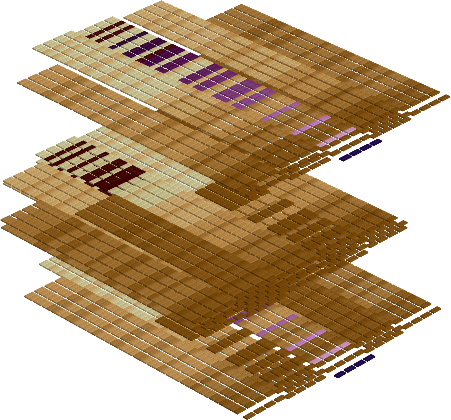
\includegraphics[width=1.5cm]{src/colorspace_colourflow/flows/colourflow_38-45.png}%           
  \end{adjustbox}                                                        
\caption*{

\begin{tikzpicture}                             
\definecolor{tempcolor}{HTML}{000000}           
\fill[tempcolor] (1 mm,0) rectangle ++(1mm,1mm);
\definecolor{tempcolor}{HTML}{975b0a}           
\fill[tempcolor] (2 mm,0) rectangle ++(1mm,1mm);
\definecolor{tempcolor}{HTML}{a86c1b}           
\fill[tempcolor] (3 mm,0) rectangle ++(1mm,1mm);
\definecolor{tempcolor}{HTML}{ca8e3d}           
\fill[tempcolor] (4 mm,0) rectangle ++(1mm,1mm);
\definecolor{tempcolor}{HTML}{ecb05f}           
\fill[tempcolor] (5 mm,0) rectangle ++(1mm,1mm);
\definecolor{tempcolor}{HTML}{ffd285}           
\fill[tempcolor] (6 mm,0) rectangle ++(1mm,1mm);
\definecolor{tempcolor}{HTML}{fff4b2}           
\fill[tempcolor] (7 mm,0) rectangle ++(1mm,1mm);
\definecolor{tempcolor}{HTML}{4f0000}           
\fill[tempcolor] (8 mm,0) rectangle ++(1mm,1mm);
\end{tikzpicture}                               
}
\end{figure}                                                               
\end{minipage}
\hspace{0.1cm}
\begin{minipage}[b]{0.15\linewidth}
\begin{figure}[H]                                                          
  \centering                                                             
  \begin{adjustbox}{width=1.5cm,center}                                   
  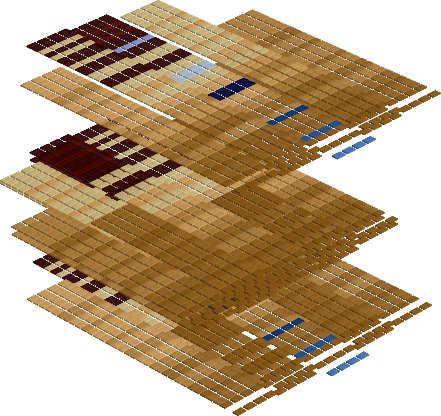
\includegraphics[width=1.5cm]{src/colorspace_colourflow/flows/colourflow_39-45.png}%           
  \end{adjustbox}                                                        
\caption*{

\begin{tikzpicture}                             
\definecolor{tempcolor}{HTML}{000000}           
\fill[tempcolor] (1 mm,0) rectangle ++(1mm,1mm);
\definecolor{tempcolor}{HTML}{a86c1b}           
\fill[tempcolor] (2 mm,0) rectangle ++(1mm,1mm);
\definecolor{tempcolor}{HTML}{b97d2c}           
\fill[tempcolor] (3 mm,0) rectangle ++(1mm,1mm);
\definecolor{tempcolor}{HTML}{db9f4e}           
\fill[tempcolor] (4 mm,0) rectangle ++(1mm,1mm);
\definecolor{tempcolor}{HTML}{fdc170}           
\fill[tempcolor] (5 mm,0) rectangle ++(1mm,1mm);
\definecolor{tempcolor}{HTML}{ffe39c}           
\fill[tempcolor] (6 mm,0) rectangle ++(1mm,1mm);
\definecolor{tempcolor}{HTML}{420404}           
\fill[tempcolor] (7 mm,0) rectangle ++(1mm,1mm);
\definecolor{tempcolor}{HTML}{600800}           
\fill[tempcolor] (8 mm,0) rectangle ++(1mm,1mm);
\end{tikzpicture}                               
}
\end{figure}                                                               
\end{minipage}
\hspace{0.1cm}
\begin{minipage}[b]{0.15\linewidth}
\begin{figure}[H]                                                          
  \centering                                                             
  \begin{adjustbox}{width=1.5cm,center}                                   
  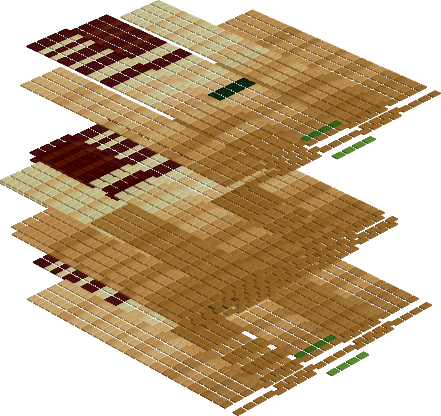
\includegraphics[width=1.5cm]{src/colorspace_colourflow/flows/colourflow_40-45.png}%           
  \end{adjustbox}                                                        
\caption*{

\begin{tikzpicture}                             
\definecolor{tempcolor}{HTML}{000000}           
\fill[tempcolor] (1 mm,0) rectangle ++(1mm,1mm);
\definecolor{tempcolor}{HTML}{b97d2c}           
\fill[tempcolor] (2 mm,0) rectangle ++(1mm,1mm);
\definecolor{tempcolor}{HTML}{ca8e3d}           
\fill[tempcolor] (3 mm,0) rectangle ++(1mm,1mm);
\definecolor{tempcolor}{HTML}{ecb05f}           
\fill[tempcolor] (4 mm,0) rectangle ++(1mm,1mm);
\definecolor{tempcolor}{HTML}{ffd285}           
\fill[tempcolor] (5 mm,0) rectangle ++(1mm,1mm);
\definecolor{tempcolor}{HTML}{fff4b2}           
\fill[tempcolor] (6 mm,0) rectangle ++(1mm,1mm);
\definecolor{tempcolor}{HTML}{4f0000}           
\fill[tempcolor] (7 mm,0) rectangle ++(1mm,1mm);
\definecolor{tempcolor}{HTML}{711900}           
\fill[tempcolor] (8 mm,0) rectangle ++(1mm,1mm);
\end{tikzpicture}                               
}
\end{figure}                                                               
\end{minipage}
\hspace{0.1cm}
\begin{minipage}[b]{0.15\linewidth}
\begin{figure}[H]                                                          
  \centering                                                             
  \begin{adjustbox}{width=1.5cm,center}                                   
  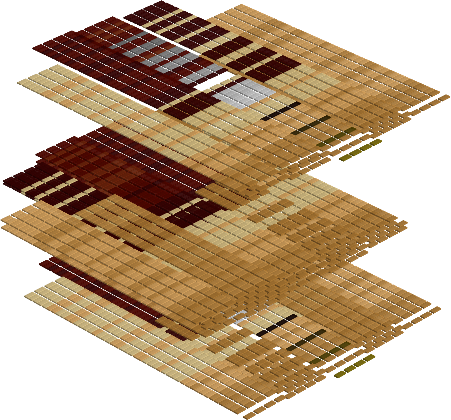
\includegraphics[width=1.5cm]{src/colorspace_colourflow/flows/colourflow_41-45.png}%           
  \end{adjustbox}                                                        
\caption*{

\begin{tikzpicture}                             
\definecolor{tempcolor}{HTML}{000000}           
\fill[tempcolor] (1 mm,0) rectangle ++(1mm,1mm);
\definecolor{tempcolor}{HTML}{ca8e3d}           
\fill[tempcolor] (2 mm,0) rectangle ++(1mm,1mm);
\definecolor{tempcolor}{HTML}{db9f4e}           
\fill[tempcolor] (3 mm,0) rectangle ++(1mm,1mm);
\definecolor{tempcolor}{HTML}{fdc170}           
\fill[tempcolor] (4 mm,0) rectangle ++(1mm,1mm);
\definecolor{tempcolor}{HTML}{ffe39c}           
\fill[tempcolor] (5 mm,0) rectangle ++(1mm,1mm);
\definecolor{tempcolor}{HTML}{420404}           
\fill[tempcolor] (6 mm,0) rectangle ++(1mm,1mm);
\definecolor{tempcolor}{HTML}{600800}           
\fill[tempcolor] (7 mm,0) rectangle ++(1mm,1mm);
\definecolor{tempcolor}{HTML}{822a0d}           
\fill[tempcolor] (8 mm,0) rectangle ++(1mm,1mm);
\end{tikzpicture}                               
}
\end{figure}                                                               
\end{minipage}
